\chapter{Créer une animation}
{ }\hfill\textbf{Niveau:} moyen\\ \\
Ce chapitre propose deux thèmes assez différents dont l'objectif est de créer une animation à l'aide de \xlogo.
\section{Les chiffres de calculatrice}
\begin{center}
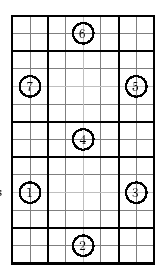
\includegraphics{images/animation-chiffre.png}
\end{center}

\noindent Cette activité est basé sur le fait que tous les nombres de calculatrice peuvent être obtenus à l'aide du patron ci-contre:
\begin{itemize}
\item Par exemple, pour dessiner un \og 4\fg, on allumera les rectangles 3,4,5,7.
\item Pour dessiner un \og 8\fg, on allumera les rectangles 1,2,3,4,5,6,7.
\item Pour dessiner un \og 3\fg, on allumera les rectangles 2,3,4,5,6.
\end{itemize}

\subsection{Remplir un rectangle}
\begin{center}
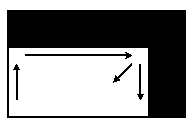
\includegraphics{images/animation-rectangle.png}
\end{center}
\noindent Si l'on souhaite par exemple tracer un rectangle rempli de 100 sur 200, une première idée peut être de dessiner le rectangle de 100 sur 200 puis de tracer un rectangle de 99 sur 199 puis un rectangle de 98 sur 198 ... jusqu'à ce que le rectangle soit entièrement rempli.  \\
Commençons par définir un rectangle de longueur et largeur dépendant de deux variables. 
\begin{verbatim}
pour rec :lo :la
repete 2[av :lo td 90 av :la td 90]
fin
\end{verbatim}
Pour remplir notre grand rectangle, on va donc exécuter:\\
\texttt{rec 100 200 rec 99 199 rec 98 198  ..... rec 1 101}\\ \\
Définissons alors une procédure rectangle dédié à tracer ce rectangle rempli.
\begin{verbatim}
pour rectangle :lo :la
rec :lo :la
rectangle :lo-1 :la-1
fin
\end{verbatim}
On teste \texttt{rectangle 100 200} et on s'aperçoit qu'il y a un problème: la procédure ne s'arrête pas lorsque le rectangle est rempli, elle continue de tracer des rectangles! On va donc ajouter un test permettant de détecter si la longueur ou la largeur est égale à 0. A ce moment, on demande au programme de s'interrompre avec la commande \texttt{stop}.
\begin{verbatim}
pour rectangle :lo :la
si ou :lo=0 :la=0 [stop]
rec :lo :la
rectangle :lo-1 :la-1
fin
\end{verbatim}
Note: à la place d'utiliser la primitive \texttt{ou}, on peut utiliser le symbole \og | \fg: on obtiendrait: \begin{center}
\texttt{si :lo=0 | :la=0 [stop]}
\end{center}

\subsection{Le programme}
\noindent Nous avons besoin du rectangle rempli précédent:
\begin{verbatim}
pour rec :lo :la
si :lo=0 |:la=0[stop]
repete 2[av :lo td 90 av :la td 90]
rec :lo-1 :la-1
fin
\end{verbatim}
Nous supposons ici que la tortue part du coin inférieur gauche. Nous allons définir une procédure appelée \texttt{chiffre} admettant 7 argument \texttt{:a}, \texttt{:b}, \texttt{:c}, \texttt{:d}, \texttt{:e}, \texttt{:f}, \texttt{:g}. Quand \texttt{:a} vaut 1, on dessine le rectangle 1. Si \texttt{:a} vaut 0, on ne le dessine pas. Voilà le principe.\\ \\
On obtient la procédure suivante:
\begin{verbatim}
pour chiffre :a :b :c :d :e :f :g
# On dessine le rectangle 1
si :a=1 [rec 160 40]
# On dessine le rectangle 2
si :b=1 [rec 40 160]
lc td 90 av 120 tg 90 bc
# On dessine le rectangle 3
si :c=1 [rec 160 40]
lc av 120 bc
# On dessine le rectangle 5
si :e=1 [rec 160 40]
# On dessine le rectangle 4
tg 90 lc re 40 bc
si :d=1 [rec 160 40]
# On dessine le rectangle 6
td 90 lc av 120 tg 90 bc
si :f=1 [rec 160 40]
# On dessine le rectangle 7
lc av 120 tg 90 re 40 bc 
si :g=1 [rec 160 40]
fin
\end{verbatim}
\subsection{Création d'une petite animation}
\noindent Nous allons ici simuler un compte à rebours en faisant apparaitre succesivement les chiffres de 9 à 0 par ordre décroissant.
\begin{verbatim}
pour rebours
ve ct chiffre 0 1 1 1 1 1 1 attends 60
ve ct chiffre 1 1 1 1 1 1 1 attends 60
ve ct chiffre 0 0 1 0 1 1 0 attends 60
ve ct chiffre 1 1 1 1 0 1 1 attends 60
ve ct chiffre 0 1 1 1 0 1 1 attends 60
ve ct chiffre 0 0 1 1 1 0 1 attends 60
ve ct chiffre 0 1 1 1 1 1 0 attends 60
ve ct chiffre 1 1 0 1 1 1 0 attends 60
ve ct chiffre 0 0 1 0 1 0 0 attends 60
ve ct chiffre 1 1 1 0 1 1 1 attends 60
fin
\end{verbatim}
Petit problème: il y a un effet de clignotement désagréable pendant la création de chaque chiffre. Pour fluidifier cela on va utiliser les primitives \texttt{animation}, \texttt{stopanimation} et \texttt{rafraichis}.\\
\begin{itemize}
\item \texttt{animation} permet de basculer en mode \og animation \fg. La tortue ne dessine plus à l'écran mais dans le cache, c'est à dire qu'elle effectue les changements en mémoire. Elle n'affichera l'image que lorsqu'on lui le demande à l'aide la primitive \texttt{rafraichis}.
\item  \texttt{stopanimation} permet de revenir à l'affichage classique.
\end{itemize}
On obtient ainsi le programme modifié:
\begin{verbatim}
pour rebours
# On passe en mode animation
animation
ve ct chiffre 0 1 1 1 1 1 1 rafraichis attends 60
ve ct chiffre 1 1 1 1 1 1 1 rafraichis attends 60
ve ct chiffre 0 0 1 0 1 1 0 rafraichis attends 60
ve ct chiffre 1 1 1 1 0 1 1 rafraichis attends 60
ve ct chiffre 0 1 1 1 0 1 1 rafraichis attends 60
ve ct chiffre 0 0 1 1 1 0 1 rafraichis attends 60
ve ct chiffre 0 1 1 1 1 1 0 rafraichis attends 60
ve ct chiffre 1 1 0 1 1 1 0 rafraichis attends 60
ve ct chiffre 0 0 1 0 1 0 0 rafraichis attends 60
ve ct chiffre 1 1 1 0 1 1 1 rafraichis attends 60
# On rebascule en mode dessin classique
stopanimation
fin
\end{verbatim}
\section{Une animation: le bonhomme qui grandit}
\begin{center}
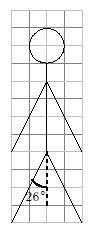
\includegraphics{images/animation-bonhomme.png}
\end{center}
Tout d'abord, nous allons définir une procédure \texttt{bon} qui trace le bonhomme ci-contre à la taille de notre choix. 
\begin{verbatim}
pour bon :c
tg 154 av 44*:c re 44*:c 
tg 52 av 44*:c re 44*:c 
tg 154 av 40*:c
tg 154 av 44*:c re :c*44 
tg 52 av 44*:c re :c*44 
tg 154 av 10*:c
tg 90 repete 180[av :c/2 td 2] td 90
fin
\end{verbatim}
Nous allons à présent créer une animation donnant l'illusion que le bonhomme grandit petit à petit. Pour cela, nous allons tracer \texttt{bon 0.1} puis \texttt{bon 0.2} \texttt{bon 0.3} ... jusqu'à \texttt{bon 5}. Entre chaque tracé, on effacera l'écran. On obtient les deux procédures suivantes:
\begin{verbatim}
pour bon :c
tg 154 av 44*:c re 44*:c 
tg 52 av 44*:c re 44*:c 
tg 154 av 40*:c
tg 154 av 44*:c re :c*44 
tg 52 av 44*:c re :c*44 
tg 154 av 10*:c
tg 90 repete 180[av :c/2 td 2] td 90
si :c=5[stop]
ve ct bon :c+0.1
fin

pour demarrer
ve ct 
bon 0
fin
\end{verbatim}
Enfin, pour fluidifier le tout, on va se servir du mode animation et de la primitive \texttt{rafraichis}.
\begin{verbatim}
pour bon :c
tg 154 av 44*:c re 44*:c 
tg 52 av 44*:c re 44*:c 
tg 154 av 40*:c
tg 154 av 44*:c re :c*44 
tg 52 av 44*:c re :c*44 
tg 154 av 10*:c
tg 90 repete 180[av :c/2 td 2] td 90
rafraichis
si :c=5[stop]
ve ct bon :c+0.1
fin

pour demarrer
ct animation
bon 0
stopanimation
fin

\end{verbatim}
\textbf{Remarque: } Ici, la procédure \texttt{bon} est récursive, on aurait plus simplement utiliser la primitive \texttt{repetepour} afin de faire varier \texttt{:c} de 0,1 à 5. Voici le programme obtenu alors:
\begin{verbatim}
pour bon :c
ve ct tg 154 av 44*:c re 44*:c 
tg 52 av 44*:c re 44*:c 
tg 154 av 40*:c
tg 154 av 44*:c re :c*44 
tg 52 av 44*:c re :c*44 
tg 154 av 10*:c
tg 90 repete 180[av :c/2 td 2] td 90
rafraichis
fin

pour demarrer
ct animation
repetepour [c 0 5 0.1][bon :c]
stopanimation
fin

\end{verbatim}

